\section{Popis algoritmů}

\subsection{2D Delaunay triangulace}
Delaunayho triangulace je algoritmus používaný k vytvoření trojúhelníkové sítě (triangulace) z množiny bodů v rovině tak, aby žádný bod neležel uvnitř kružnice opsané žádnému z trojúhelníků. Výsledná triangulace má vlastnost, že maximalizuje minimální úhel všech trojúhelníků, čímž se minimalizuje výskyt trojúhelníků s ostrými úhly.\\

\hspace{-1.15cm}
Nejprve je nalezen bod $p_1$ který má minimální $x$ souřadnici: 
\begin{equation}
    p_1 = \text{min}(x_i)
\end{equation}
Následně je vybrán bod $p_2$ který se nachází nejblíže bodu $p_2$:
\begin{equation}
    p_2 = \text{min}(s_{p_1,p_2})
\end{equation}
Následně byla vytvořena hrana $e_1$, která je tvořena body $p_1,p_2$ a hrana $e_2$ kterou tvoří stejné body, ale s opačnou orientací tudíž $p_2,p_1$
Hrany jsou přidány do pomocné konstrukce $AEL$
\begin{equation}
    AEL.\text{push\_back}(e_1,e_2)
\end{equation}
Prochází se proměnou $AEL$ dokud není prázdná. Vezme se první hrana a změní se její orientace. Prochází se pouze body, které leží vpravo od hrany. Dále se najde bod, který s počátečním a koncovým bodem hrany svírá největší úhel. Takovému bodu se říká Delauayovský bod:
\begin{equation}
    p_{d} = \text{max} \angle( p_{d},p_{\text{end}},p_d,p_{\text{start}})
\end{equation}
Pokud se takový bod najde, všechny hrany jsou přidány do $DT$:
\begin{equation}
    dt.\text{push\_back}(e_{1},e_{p_1,d},e_{p_2,d})
\end{equation}
Nakonec je zkontrolováno zda se hrana s opačnou orientací nenachází v $AEL$. Pokud ano hrana s opačnou orientací je odstraněna z $AEL$, pokud ne hrana je přidána do $AEL$ 

\begin{algorithm}
    \setstretch{0.8}
    \caption{Metoda \texttt{DT} -- Delaunayova triangulace (inkrementálně)}
    \begin{algorithmic}[1]
        \STATE \textbf{Vstup:} množina bodů $P$
        \STATE \textbf{Výstup:} množina hran Delaunayovy triangulace $\text{DT}$

        \STATE $\text{DT} \gets \emptyset$ \COMMENT{výsledná triangulace}
        \STATE $\text{AEL} \gets \emptyset$ \COMMENT{aktivní hrany (Active Edge List)}

        \STATE $p_1 \gets \text{nejlevější bod z } P$ \COMMENT{pivot podle $x$-ové souřadnice}
        \STATE $p_2 \gets \text{nejbližší bod k } p_1 \text{ z } P$

        \STATE $e_1 \gets (p_1, p_2)$
        \STATE $e_2 \gets (p_2, p_1)$

        \STATE přidej $e_1$, $e_2$ do $\text{AEL}$

        \WHILE{$\text{AEL} \neq \emptyset$}
            \STATE $e \gets$ poslední prvek z $\text{AEL}$
            \STATE odstraň $e$ z $\text{AEL}$

            \STATE $e_s \gets$ změň orientaci hrany $e$

            \STATE $p_d \gets \text{findDelaunayPoint}(e_s.\text{start}, e_s.\text{end}, P)$

            \IF{$p_d \neq \texttt{null}$}
                \STATE $e_2s \gets (e_s.\text{end}, p_d)$
                \STATE $e_3s \gets (p_d, e_s.\text{start})$

                \STATE přidej $e_s$, $e_2s$, $e_3s$ do $\text{DT}$

                \STATE \text{updateAEL}$(e_2s, \text{AEL})$
                \STATE \text{updateAEL}$(e_3s, \text{AEL})$
            \ENDIF
        \ENDWHILE

        \STATE \textbf{return} $\text{DT}$
    \end{algorithmic}
\end{algorithm}

\begin{algorithm}
    \setstretch{0.8}
    \caption{Metoda \texttt{getPointAndLinePosition}}
    \begin{algorithmic}[1]
        \STATE \textbf{Vstup:} bod $p$, počáteční bod $p_1$, koncový bod $p_2$
        \STATE \textbf{Výstup:} pozice bodu $p$ vůči orientované přímce $(p_1, p_2)$
        \STATE \textbf{Návratové hodnoty:} 
        \begin{itemize}
            \item $1$ pokud je bod $p$ vlevo od přímky
            \item $0$ pokud je bod $p$ vpravo od přímky
            \item $-1$ pokud leží na přímce
        \end{itemize}

        \STATE $\varepsilon \gets 10^{-6}$

        \STATE $u_x \gets p_2.x - p_1.x$
        \STATE $u_y \gets p_2.y - p_1.y$

        \STATE $v_x \gets p.x - p_1.x$
        \STATE $v_y \gets p.y - p_1.y$

        \STATE $t \gets u_x \cdot v_y - u_y \cdot v_x$ \COMMENT{determinant pro orientaci}

        \IF{$t > \varepsilon$}
            \STATE \textbf{return} $1$
        \ELSIF{$t < -\varepsilon$}
            \STATE \textbf{return} $0$
        \ELSE
            \STATE \textbf{return} $-1$
        \ENDIF
    \end{algorithmic}
\end{algorithm}


\begin{algorithm}
    \setstretch{0.8}
    \caption{Metoda \texttt{get2LinesAngle}}
    \begin{algorithmic}[1]
        \STATE \textbf{Vstup:} body $p_1$, $p_2$ definující první přímku a $p_3$, $p_4$ definující druhou přímku
        \STATE \textbf{Výstup:} úhel mezi přímkami v radiánech

        \STATE $u_x \gets p_2.x - p_1.x$
        \STATE $u_y \gets p_2.y - p_1.y$
        \STATE $v_x \gets p_4.x - p_3.x$
        \STATE $v_y \gets p_4.y - p_3.y$

        \STATE $\text{skalární součin } \gets u_x \cdot v_x + u_y \cdot v_y$

        \STATE $n_u \gets \sqrt{u_x^2 + u_y^2}$ \COMMENT{norma vektoru $u$}
        \STATE $n_v \gets \sqrt{v_x^2 + v_y^2}$ \COMMENT{norma vektoru $v$}

        \STATE \textbf{return} $\arccos\left(\dfrac{\text{skalární součin}}{n_u \cdot n_v}\right)$
    \end{algorithmic}
\end{algorithm}


\begin{algorithm}
    \setstretch{0.8}
    \caption{Metoda \texttt{findDelaunayPoint}}
    \begin{algorithmic}[1]
        \STATE \textbf{Vstup:} body $p_1$, $p_2$, množina bodů $P$
        \STATE \textbf{Výstup:} index bodu $p_d \in P$, který tvoří největší úhel $\angle p_1 p_d p_2$ a leží vlevo od přímky $(p_1, p_2)$

        \STATE $i_{\max} \gets -1$ \COMMENT{žádný bod zatím nebyl nalezen}
        \STATE $\omega_{\max} \gets 0$

        \FOR{$i \gets 0$ \TO $\text{size}(P) - 1$}
            \IF{\texttt{getPointAndLinePosition}$(P[i], p_1, p_2) = 1$}
                \STATE $\omega \gets$ \texttt{get2LinesAngle}$(P[i], p_1, P[i], p_2)$
                \IF{$\omega > \omega_{\max}$}
                    \STATE $\omega_{\max} \gets \omega$
                    \STATE $i_{\max} \gets i$
                \ENDIF
            \ENDIF
        \ENDFOR

        \STATE \textbf{return} $i_{\max}$
    \end{algorithmic}
\end{algorithm}


\begin{algorithm}
    \setstretch{0.8}
    \caption{Metoda \texttt{get2DDistance}}
    \begin{algorithmic}[1]
        \STATE \textbf{Vstup:} body $p_1$, $p_2$
        \STATE \textbf{Výstup:} 2D eukleidovská vzdálenost mezi body $p_1$ a $p_2$

        \STATE $dx \gets p_1.x - p_2.x$
        \STATE $dy \gets p_1.y - p_2.y$

        \STATE \textbf{return} $\sqrt{dx^2 + dy^2}$
    \end{algorithmic}
\end{algorithm}


\begin{algorithm}
    \setstretch{0.8}
    \caption{Metoda \texttt{findNearestPoint}}
    \begin{algorithmic}[1]
        \STATE \textbf{Vstup:} bod $p$, množina bodů $P$
        \STATE \textbf{Výstup:} index bodu $p_{\min} \in P$, který je nejblíže bodu $p$

        \STATE $i_{\min} \gets -1$
        \STATE $\varepsilon \gets 10^{-16}$ \COMMENT{tolerance pro porovnání}
        \STATE $d_{\min} \gets 10^{16}$ \COMMENT{počáteční nekonečná vzdálenost}

        \FOR{$i \gets 0$ \TO $\text{size}(P) - 1$}
            \IF{$p \neq P[i]$}
                \STATE $d \gets$ \texttt{get2DDistance}$(p, P[i])$
                \IF{$d < d_{\min}$}
                    \STATE $d_{\min} \gets d$
                    \STATE $i_{\min} \gets i$
                \ENDIF
            \ENDIF
        \ENDFOR

        \STATE \textbf{return} $i_{\min}$
    \end{algorithmic}
\end{algorithm}

\begin{algorithm}
    \setstretch{0.8}
    \caption{Metoda \texttt{updateAEL}}
    \begin{algorithmic}[1]
        \STATE \textbf{Vstup:} hrana $e$, seznam aktivních hran \texttt{AEL}
        \STATE \textbf{Výstup:} aktualizovaný seznam \texttt{AEL}

        \STATE $e_s \gets$ \texttt{changeOrientation}$(e)$ \COMMENT{změní orientaci hrany}

        \STATE $i_e \gets$ index hrany $e_s$ v \texttt{AEL} \COMMENT{vyhledání opačné hrany}

        \IF{$e_s$ \textbf{není nalezena} v \texttt{AEL}}
            \STATE přidej $e$ do \texttt{AEL} \COMMENT{hrana je nová, trojúhelník vzniká poprvé}
        \ELSE
            \STATE odstraň $e_s$ z \texttt{AEL} \COMMENT{opačná hrana už existuje, trojúhelník je kompletní}
        \ENDIF
    \end{algorithmic}
\end{algorithm}


\newpage
\subsection{Tvorba vrstevnic}
Je algoritmus, který za použití lineární interpolace vytváří vrstevnice z Delaunayova triangulace.\\

\hspace{-1.15cm}
\begin{equation}
    x_a = \frac{x_3-x_1}{z_3-z_1}(z-z_1)+x_1;~
    y_a = \frac{y_3-y_1}{z_3-z_1}(z-z_1)+y_1
\end{equation}
Vrstevnice jsou reprezentovány pomocí vektoru hran. Při výpočtu se pracuje na intervalu od $z_{min}$ do $z_{max}$ s krokem $\delta_z$. V prvním kroku se vybere první trojúhelník vytvořený Delaunayovou triangulací:
\begin{equation}
    p_1 = dt{i};~
    p_2 = dt_{i+1};~
    p_3 = dt_{i+3}
\end{equation}
Od aktuální hodnoty z jsou odečteny hodnoty jednotlivých bodů:
\begin{equation}
    \delta_{z_1} = z-p_{1z};~
    \delta_{z_2} = z-p_{2z};~
    \delta_{z_3} = z-p_{3z}
\end{equation}
Před výpočtem souřadnic $x$ a $y$ je nutné ověřit, jak je umístěn trojúhelník v prostoru vůči rovině tvořenou souřadnicí z. Pokud $\delta_{z_1}$, $\delta_{z_2}$ a $\delta_{z_3}$ jsou všechny rovny nule trojúhelník je koplanární proto ho není potřeba řešit. Pokud dvojice rozdílů je rovna 0, hrana tvoří vrstevnici. V ostatních případech násobky rozdílů:
\begin{equation}
    \delta_{z_1}\delta_{z_2};~
    \delta_{z_1}\delta_{z_3};~
    \delta_{z_2}\delta_{z_3}
\end{equation}
Pomocí lineární interpolace se vypočítají souřadnice průsečíku pouze v případě, že násobek je $< 0$. V ostatních případech výpočet nemá smysl.
\begin{algorithm}
    \setstretch{0.8}
    \caption{Metoda \texttt{createContourLines}}
    \begin{algorithmic}[1]
        \STATE \textbf{Vstup:} triangulace \texttt{dt}, minimální výška $z_{\min}$, maximální výška $z_{\max}$, krok $dz$
        \STATE \textbf{Výstup:} seznam vrstevnicových hran \texttt{contour\_lines}

        \STATE \texttt{contour\_lines} $\gets \emptyset$

        \FOR{$z \gets z_{\min}$ \TO $z_{\max}$ s krokem $dz$}
            \FOR{$i \gets 0$ \TO $\text{size}(dt) - 1$ po třech}
                \STATE $p_1 \gets \text{start}(dt[i])$
                \STATE $p_2 \gets \text{start}(dt[i+1])$
                \STATE $p_3 \gets \text{start}(dt[i+2])$

                \STATE $dz_1 \gets z - p_1.z$
                \STATE $dz_2 \gets z - p_2.z$
                \STATE $dz_3 \gets z - p_3.z$

                \IF{$dz_1 = 0$ \AND $dz_2 = 0$}
                    \STATE přidej $dt[i]$ do \texttt{contour\_lines}
                    \STATE \textbf{continue}
                \ENDIF
                \IF{$dz_2 = 0$ \AND $dz_3 = 0$}
                    \STATE přidej $dt[i+1]$ do \texttt{contour\_lines}
                    \STATE \textbf{continue}
                \ENDIF
                \IF{$dz_3 = 0$ \AND $dz_1 = 0$}
                    \STATE přidej $dt[i+2]$ do \texttt{contour\_lines}
                    \STATE \textbf{continue}
                \ENDIF

                \IF{$dz_1 \cdot dz_2 \leq 0$}
                    \STATE $a \gets \texttt{countourLinePoint}(p_1, p_2, z)$
                    \IF{$dz_2 \cdot dz_3 \leq 0$}
                        \STATE $b \gets \texttt{countourLinePoint}(p_2, p_3, z)$
                        \STATE přidej hranu $(a, b)$ do \texttt{contour\_lines}
                    \ELSIF{$dz_3 \cdot dz_1 \leq 0$}
                        \STATE $b \gets \texttt{countourLinePoint}(p_3, p_1, z)$
                        \STATE přidej hranu $(a, b)$ do \texttt{contour\_lines}
                    \ENDIF
                \ELSIF{$dz_2 \cdot dz_3 \leq 0$}
                    \STATE $a \gets \texttt{countourLinePoint}(p_2, p_3, z)$
                    \IF{$dz_3 \cdot dz_1 \leq 0$}
                        \STATE $b \gets \texttt{countourLinePoint}(p_3, p_1, z)$
                        \STATE přidej hranu $(a, b)$ do \texttt{contour\_lines}
                    \ENDIF
                \ENDIF
            \ENDFOR
        \ENDFOR

        \STATE \textbf{return} \texttt{contour\_lines}
    \end{algorithmic}
\end{algorithm}

\begin{algorithm}
    \setstretch{0.8}
    \caption{Metoda \texttt{countourLinePoint}}
    \begin{algorithmic}[1]
        \STATE \textbf{Vstup:} body $p_1$, $p_2$, výšková hodnota $z$
        \STATE \textbf{Výstup:} bod $p$ na vrstevnici $z$ mezi $p_1$ a $p_2$

        \STATE $x_b \gets \left(\dfrac{p_2.x - p_1.x}{p_2.z - p_1.z}\right) \cdot (z - p_1.z) + p_1.x$
        \STATE $y_b \gets \left(\dfrac{p_2.y - p_1.y}{p_2.z - p_1.z}\right) \cdot (z - p_1.z) + p_1.y$

        \STATE \textbf{return} bod $(x_b, y_b, z)$
    \end{algorithmic}
\end{algorithm}


\newpage

\subsection{Analýza sklonu}
Pro jednotlivé trojúhelníky je vypočítán sklon daného trojúhelníku.\\

\hspace{-1.15cm}
Pokud je vektor trojúhelníků prázdný, nebo byly přidány nové body, je přepočítán vektor trojúhelníků. Z třech bodů trojúhelníku  $p_1 = (x_1, y_1, z_1)$, $p_2 = (x_2, y_2, z_2)$ a $p_3 = (x_3, y_3, z_3)$.

\begin{equation}
\vec{u} = (x_3 - x_2,\, y_3 - y_2,\, z_3 - z_2)
\end{equation}

\begin{equation}
\vec{v} = (x_1 - x_2,\, y_1 - y_2,\, z_1 - z_2)
\end{equation}

Normálový vektor $\vec{n}$ je určen jako vektorový součin $\vec{u} \times \vec{v}$:

\begin{equation}
n_x = (y_3 - y_2)(z_1 - z_2) - (z_3 - z_2)(y_1 - y_2)
\end{equation}

\begin{equation}
n_y = -\left[(x_3 - x_2)(z_1 - z_2) - (z_3 - z_2)(x_1 - x_2)\right]
\end{equation}

\begin{equation}
n_z = (x_3 - x_2)(y_1 - y_2) - (y_3 - y_2)(x_1 - x_2)
\end{equation}

Velikost normálového vektoru:

\begin{equation}
\|\vec{n}\| = \sqrt{n_x^2 + n_y^2 + n_z^2}
\end{equation}

Sklon trojúhelníka vůči rovině XY (v radiánech):

\begin{equation}
\theta = \arccos\left( \frac{n_z}{\|\vec{n}\|} \right)
\end{equation}

Pro zobrazení sklonu svahu byla použita barevná stupnice v odstínech šedi. Kdy nejmenší sklon zobrazuje bílá barva a největší sklon černá barva.
\begin{algorithm}
    \setstretch{0.9}
    \caption{Metoda \texttt{edgesToTriangle}}
    \begin{algorithmic}[1]
        \STATE \textbf{Vstup:} seznam hran triangulace \texttt{dt}
        \STATE \textbf{Výstup:} seznam trojúhelníků \texttt{triangles}

        \FOR{$i \gets 0$ \TO $\text{size}(dt) - 1$ po třech}
            \STATE $p_1 \gets \text{start}(dt[i])$
            \STATE $p_2 \gets \text{start}(dt[i+1])$
            \STATE $p_3 \gets \text{start}(dt[i+2])$

            \STATE $t \gets \text{nový trojúhelník}(p_1, p_2, p_3)$

            \STATE přidej $t$ do \texttt{triangles}
        \ENDFOR
    \end{algorithmic}
\end{algorithm}

\begin{algorithm}
    \setstretch{0.9}
    \caption{Metoda \texttt{analyzeSlope}}
    \begin{algorithmic}[1]
        \STATE \textbf{Vstup:} triangulace \texttt{dt}, seznam trojúhelníků \texttt{triangles}, boolean \texttt{click}
        \STATE \textbf{Výstup:} aktualizovaný seznam \texttt{triangles} s hodnotami sklonu

        \IF{$\text{size}(triangles) = 0$ \OR click}
            \STATE \text{edgesToTriangle}(dt, triangles)
        \ENDIF

        \FOR{$i \gets 0$ \TO $\text{size}(triangles) - 1$}
            \STATE $p_1 \gets \text{triangles}[i].\text{getP1()}$
            \STATE $p_2 \gets \text{triangles}[i].\text{getP2()}$
            \STATE $p_3 \gets \text{triangles}[i].\text{getP3()}$

            \STATE $s \gets \text{computeSlope}(p_1, p_2, p_3)$

            \STATE \text{triangles}[i].\text{setSlope}$(s)$
        \ENDFOR
    \end{algorithmic}
\end{algorithm}

\begin{algorithm}
    \setstretch{0.9}
    \caption{Metoda \texttt{computeSlope}}
    \begin{algorithmic}[1]
        \STATE \textbf{Vstup:} body $p_1$, $p_2$, $p_3$
        \STATE \textbf{Výstup:} sklon trojúhelníku v radiánech

        \STATE $u \gets \vec{p_2p_3} = (u_x, u_y, u_z) = (p_3.x - p_2.x,\ p_3.y - p_2.y,\ p_3.z - p_2.z)$
        \STATE $v \gets \vec{p_2p_1} = (v_x, v_y, v_z) = (p_1.x - p_2.x,\ p_1.y - p_2.y,\ p_1.z - p_2.z)$

        \STATE $n_x \gets u_y \cdot v_z - u_z \cdot v_y$
        \STATE $n_y \gets -(u_x \cdot v_z - u_z \cdot v_x)$
        \STATE $n_z \gets u_x \cdot v_y - u_y \cdot v_x$

        \STATE $n \gets \sqrt{n_x^2 + n_y^2 + n_z^2}$ \COMMENT{velikost normálového vektoru}

        \STATE \textbf{return} $\arccos \left(\dfrac{n_z}{n}\right)$
    \end{algorithmic}
\end{algorithm}


\subsection{Orientace svahu}
Pro jednotlivé trojúhelníky je vypočítána orientace daného trojúhelníku.\\

\hspace{-1.15cm}
Pokud je vektor trojúhelníků prázdný, nebo byly přidány nové body, je přepočítán vektor trojúhelníků. Z třech bodů trojúhelníku  $p_1 = (x_1, y_1, z_1)$, $p_2 = (x_2, y_2, z_2)$ a $p_3 = (x_3, y_3, z_3)$.

\begin{equation}
\vec{u} = (x_3 - x_2,\, y_3 - y_2,\, z_3 - z_2)
\end{equation}

\begin{equation}
\vec{v} = (x_1 - x_2,\, y_1 - y_2,\, z_1 - z_2)
\end{equation}

Normálový vektor $\vec{n}$ je určen jako vektorový součin $\vec{u} \times \vec{v}$:

\begin{equation}
n_x = (y_3 - y_2)(z_1 - z_2) - (z_3 - z_2)(y_1 - y_2)
\end{equation}

\begin{equation}
n_y = -\left[(x_3 - x_2)(z_1 - z_2) - (z_3 - z_2)(x_1 - x_2)\right]
\end{equation}

\begin{equation}
n_z = (x_3 - x_2)(y_1 - y_2) - (y_3 - y_2)(x_1 - x_2)
\end{equation}

Velikost normálového vektoru:

\begin{equation}
\|\vec{n}\| = \sqrt{n_x^2 + n_y^2 + n_z^2}
\end{equation}

Orientace trojúhelníka vůči rovině XY (v radiánech):

\begin{equation}
\theta = \arctan2\left( \frac{n_z}{\|\vec{n}\|} \right)
\end{equation}


Pro zobrazení orientace trojúhelníku byla využita tato barevná stupnice: \\
\begin{figure}[H]
  \centering
  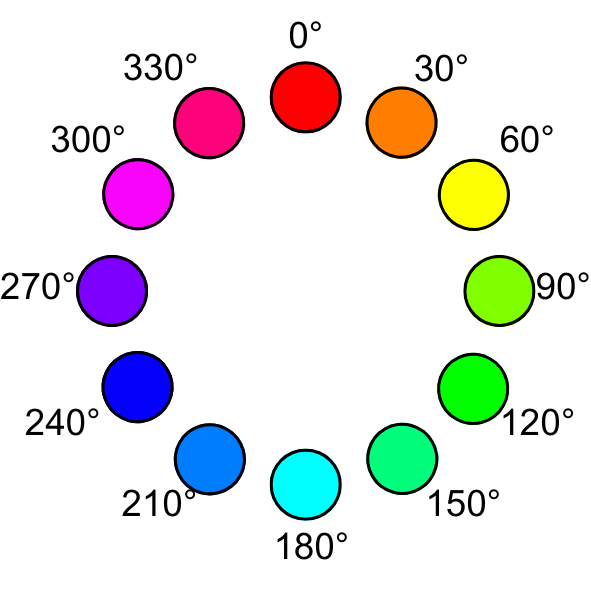
\includegraphics[width=0.3\textwidth]{images/Colorwheel.png}
  \caption{Barevná stupnice}
\end{figure}

\begin{algorithm}
    \setstretch{0.9}
    \caption{Metoda \texttt{analyzeAspect}}
    \begin{algorithmic}[1]
        \STATE \textbf{Vstup:} triangulace \texttt{dt}, seznam trojúhelníků \texttt{triangles}, boolean \texttt{click}
        \STATE \textbf{Výstup:} aktualizovaný seznam \texttt{triangles} s hodnotami orientace

        \IF{$\text{size}(triangles) = 0$ \OR click}
            \STATE \text{edgesToTriangle}(dt, triangles)
        \ENDIF

        \FOR{$i \gets 0$ \TO $\text{size}(triangles) - 1$}
            \STATE $p_1 \gets \text{triangles}[i].\text{getP1()}$
            \STATE $p_2 \gets \text{triangles}[i].\text{getP2()}$
            \STATE $p_3 \gets \text{triangles}[i].\text{getP3()}$

            \STATE $a \gets \text{computeAspect}(p_1, p_2, p_3)$

            \STATE \text{triangles}[i].\text{setAspect}$(a)$
        \ENDFOR
    \end{algorithmic}
\end{algorithm}

\begin{algorithm}
    \setstretch{0.9}
    \caption{Metoda \texttt{computeAspect}}
    \begin{algorithmic}[1]
        \STATE \textbf{Vstup:} body $p_1$, $p_2$, $p_3$
        \STATE \textbf{Výstup:} Orientace trojúhelníku v radiánech

        \STATE $u \gets \vec{p_2p_3} = (u_x, u_y, u_z) = (p_3.x - p_2.x,\ p_3.y - p_2.y,\ p_3.z - p_2.z)$
        \STATE $v \gets \vec{p_2p_1} = (v_x, v_y, v_z) = (p_1.x - p_2.x,\ p_1.y - p_2.y,\ p_1.z - p_2.z)$

        \STATE $n_x \gets u_y \cdot v_z - u_z \cdot v_y$
        \STATE $n_y \gets -(u_x \cdot v_z - u_z \cdot v_x)$
        \STATE $n_z \gets u_x \cdot v_y - u_y \cdot v_x$

        \STATE $n \gets \sqrt{n_x^2 + n_y^2 + n_z^2}$ \COMMENT{velikost normálového vektoru}

        \STATE \textbf{return} $\arctan2 \left(\dfrac{n_z}{n}\right)$
    \end{algorithmic}
\end{algorithm}
\subsection{Generování umělých útvarů}

Pro účely testování algoritmů byly v aplikaci implementovány funkce pro generování umělých terénních útvarů. Všechny útvary jsou generovány jako množiny náhodně rozložených bodů s výškou vypočtenou podle geometrické funkce. Cílem je generovat modelové situace, na kterých je možné sledovat chování algoritmů pro triangulaci, tvorbu vrstevnic, sklon a expozici.

\subsubsection{Kupa}
Kupa je generována jako eliptický paraboloid, kde výška je největší ve středu a klesá směrem ke krajům:
\[
z = \text{maxZ} \cdot \left(1 - \left(\frac{x - cx}{rx}\right)^2 - \left(\frac{y - cy}{ry}\right)^2\right)
\]
Pokud je výška $z < 0$, nastaví se na nulu. Výsledkem je hladký kopec soustředěný okolo bodu $(cx, cy)$ s poloměry $rx$, $ry$.

\subsubsection{Údolí}
Údolí je inverzní verzí kopce. Výška roste směrem od středu:
\[
z = \text{depth} \cdot \left(\left(\frac{x - cx}{rx}\right)^2 + \left(\frac{y - cy}{ry}\right)^2\right)
\]

\subsubsection{Hřbet}
Tvar hřbetu je určen přímkou mezi dvěma body $(x_1, y_1)$ a $(x_2, y_2)$. Výška bodu klesá lineárně s jeho kolmou vzdáleností od této osy:
\[
z = \text{maxZ} - d
\]
kde $d$ je kolmá vzdálenost bodu $(x, y)$ od přímky spojující dva body $(x_1, y_1)$ a $(x_2, y_2)$. Tato vzdálenost se počítá jako:
\[
d = \frac{|(y_2 - y_1)x - (x_2 - x_1)y + x_2 y_1 - y_2 x_1|}{\sqrt{(x_2 - x_1)^2 + (y_2 - y_1)^2}}
\]

\subsubsection{Spočinek}
Spočinek je modelován jako skok ve výšce v určitém rozsahu souřadnice $x$. Všechny body mají výšku 1000, ale pokud $x$ leží v intervalu $(\text{stepStartX}, \text{stepEndX})$, výška se sníží o hodnotu $depthZ$:
\[
z = \begin{cases}
1000 - \text{depthZ} & \text{pokud } x \in (\text{stepStartX}, \text{stepEndX}) \\
1000 & \text{jinak}
\end{cases}
\]
Tím vzniká ostrý zlom v terénu.

\subsubsection{Sedlo}
Sedlo je generováno jako hyperbolický paraboloid:
\[
z = 500 + 10 \cdot \left(\left(\frac{x - cx}{scaleX}\right)^2 - \left(\frac{y - cy}{scaleY}\right)^2\right)
\]
Výsledkem jsou dva protilehlé svahy. Jeden klesající a druhý stoupající se středem v bodě $(cx, cy)$.

